\documentclass[11pt]{article}

\title{Model Checking World Domination}
\author{Jacob Errington \& Kevin Li}
\date{Formal Verification -- COMP 525\\18 April 2017}

\usepackage{tikz}
\usepackage{amsthm,amsmath,amssymb}
\usepackage{csquotes}
\usepackage[margin=3.0cm]{geometry}
\usetikzlibrary{automata}
\usetikzlibrary{graphs}

\theoremstyle{definition}
\newtheorem{defn}{Definition}

\begin{document}

\maketitle

\begin{abstract}
    % > Probabilistic model checking is employed in swarm robotics to verify
    % > properties of swarm behavior in the context of tasks.
    % TODO "in the context of tasks" sounds super vague
    %
    Probabilistic model checked is used to verify properties of a robotic swarm
    performing a certain task.
    %
    Several canonical tasks are often used in testing swarms for desired
    collective behavior, such as foraging, flocking, and navigation.
    % TODO I don't like this sentence. I'm not sure how best to rephrase it.
    %
    % > Swarms performing such tasks face numerous challenges, one of which is
    % > task allocation, which is concerned with optimal division of labour
    % > between individuals and groups of robots in a swarm.
    %
    The problem of robotic swarm task allocation arises when a swarm is
    presented with multiple tasks to complete concurrently: in what proportions
    must a swarm disaggregate and recombine to most efficiently complete all
    tasks?
    %
    Extant literature on robotic swarm task allocation focusses on the
    aforementioned types of tasks.
    %
    In this paper we introduce the notion of distributable probabilistic tasks,
    % > a class of tasks with particular traits,
    % This sounds very very vague, and can probably just be omitted
    and propose a probabilistic model checking framework through which optimal
    allocation proportions can be derived.
    %
    % > We then conduct experiments using our
    % > framework in the context of several combat scenarios,
    % > and present experimental results.
    %
    % TODO Not sure this should be said in the abstract.
\end{abstract}

\section{Introduction}
\label{sec:intro}

A robot swarm is a group of robots acting cooperatively to perform a task.
Different types of swarms have been considered in the literature.
Most often, one considers homogeneous swarms, in which the members have
identical capabilities.
Swarm robotics is a notorious field due to issues of \emph{scale}.
It is not necessarily clear what properties a swarm will have when one knows
only the properties of its members.
Contrariwise, knowing only the properties of the swarm in aggregate, it can be
difficult to see what properties the members ought to have.
Hence in the design of robot swarms, there are two major approaches:
%
\begin{enumerate}
    \item
        the \emph{macroscopic} approach focusses on the desired properties of
        the swarm as a whole, and attempts to determine how to build suitable
        member robots;
        % cite example of macroscopic approach
        %
    \item
        the \emph{microscopic} approach starts with the design of individual
        robots, and attempts to predict what properties emerge from that
        construction.
        % cite example of microscopic approach
        %
\end{enumerate}

In recent years, robot swarm engineering has evolved from a rather ad hoc
endeavor to a more principled science.
ASDF 20XX proposes a novel framework for designing robot swarms: their
methodology is driven by model checking.
% TODO cite their paper
As the outcomes of a robot's actions are uncertain, the techniques of
probabilistic model checking are more appropriate.
%
% ... "and has played a major role in the engineering of correct swarm
% behaviour." ?
% I liked this mention from the original, but we will need a citation.
% TODO decide whether to include this mention
%
% > Formal verification, and in particular probabilistic model
% > checking, has played a major role in the engineering of
% > correct swarm and individual robot behavior. % Citation needed.
% >
% > There are generally two approaches for modeling a swarm robotics
% > system: the microscopic and macroscopic view.
% >
% > In the microscopic view, the behavior of an individual robot
% > is first modeled with a transition system. Then,
% > a model corresponding to the behavior of the swarm is
% > generated by creating a composed transition system
% > by composing many of the individual transition systems
% > together. This representation is useful for verifying
% > properties of individual robots, but is not
% > very useful for the verification of properties of the
% > entire swarm when the population of robots in the swarm
% > is high, as the state space grows exponentially in
% > the number of composed transition systems.
%
% I already discuss macro vs micro above, so now I just focus on the
% application of model-checking to micro:

In applying the principles of model checking to the microscopic approach to
swarm design, one models each member of the swarm as an independent transition
system.
Communication and coordination protocols are modelled as controllers.
The swarm's behaviour can then be studied by examining the properties of the
composed transition system.
As swarms of greater size are modelled in this way, the composition of their
transition systems becomes considerably larger.
% TODO cite / explain just how much bigger?
Due to this state space explosion, microscopic model checking is currently
infeasible for swarms of any appreciable size.

% > In the macroscopic view (assuming that the robots
% > in the swarm are identical in design and can be
% > modeled with the same transition system), a single
% > transition system is used to represent the entire
% > swarm. The transition system is identical to the
% > transition system that models individual behavior of
% > a single robot, except where each state is
% > annotated with a variable that describes the
% > number of robots in the swarm that are currently
% > in that state. \cite{konur12}
%
In contrast, the macroscopic approach does not track the internal state of each
robot directly as in the microscopic approach.
Assuming a homogeneous robots, the macroscopic approach uses a single
transition system to model the swarm.
This system is obtained by considering the different states a single robot can
be in, and augmenting these states with a count of how many robots of the swarm
are in that state.
The transition rules between states in the augmented system must
govern what \emph{proportion} of robots change state without having access to
the internal details of the particular robots.

% > By representing a swarm robotics system this way,
% > we can describe a far larger swarm,
% > which makes the properties that can be verified
% > much more interesting. Thus, this is the representation
% > of a robot swarm that we will use for this paper.
%
In this paper, we follow the macroscopic approach.
By representing the robotic swarm in this way, we can describe and analyze a
much larger system than otherwise possible.
This makes it possible to verify more interesting properties.
%
The scope of this paper does not include the (daunting) challenges involved in
the engineering of a robot swarm, nor do we take into account many practical
considerations such as the reliability of communication between robots or
hardware.
We take an abstract view of a robotic swarm and assume (perhaps recklessly)
that these issues are solved.

This paper is structured as follows.
%
In section \ref{sec:background-motivation} we provide an overview of the
existing literature on probabilistic model checking and on task allocation in
swarm robotics.
We then introduce the problem domain that our framework tackles, along with
the notion of a distributable probabilistic task.
%
In section \ref{sec:model} we describe how our framework is constructed using a
concrete combat example.
%
In section \ref{sec:implementation} we describe the implementation of our
framework, along with the specifications of how our experiments were
implemented.
%
In section \ref{sec:results} we present our experimental results and discuss
their relevance.
%
We conclude in section \ref{sec:conclusion} and consider avenues for future
improvement.

\section{Background and Motivation}
\label{sec:background-motivation}

The real-world results of actions are uncertain. Thus,
probabilistic models are ideal for representing
real-world swarm robotics systems.
In particular, discrete time Markov chains (DTMCs)
are used to extend the transition system representation
of a robot swarm, to encode the effects of taking actions
that produce probabilistic results.

Liu, Winfield, and Sa represent a foraging swarm
using a discrete time Markov chain. Figure \ref{fig:foraging}
shows their construction using the macroscopic
representation of a robot swarm.

\begin{figure}
    \caption{Konur, Dixon, and Fisher's foraging swarm representation}
    \label{fig:foraging}
    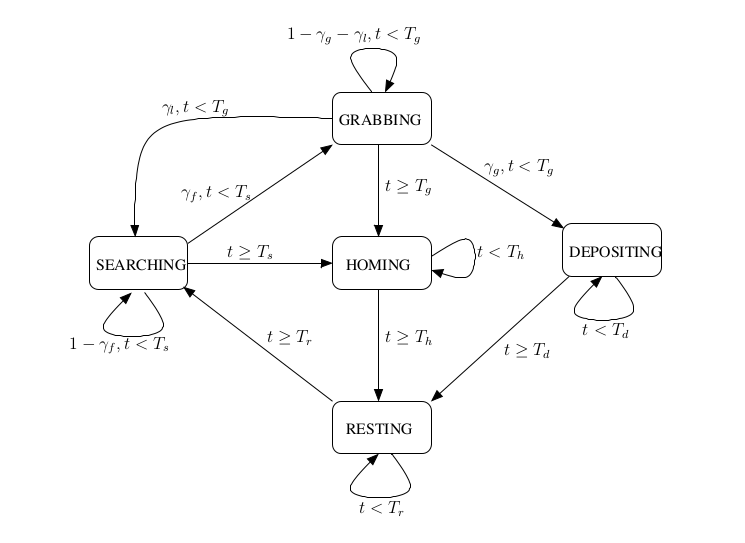
\includegraphics[width=\textwidth]{foraging.png}
\end{figure}

The macroscopic representation of this robotic swarm
shows that each robot is responsible for attempting
to gather "food" in order to increase the overall
energy levels of the entire swarm. The semantics
of the states are:

\begin{description}
    \item[Searching] Robot is searching for food
    \item[Grabbing] Robot attempts to grab a food item
    \item[Depositing] Robot returns home with the food item
    \item[Homing] Robot returns home without any food items
    \item[Resting] Robot rests for some time
\end{description}

Then, there are some timeout conditions and probability
distributions over states after a transition is performed.

\begin{itemize}
    \item $ T_s $ is the maximum amount time a robot can continue searching.
    \item $ T_g $ is the maximum amount of time a robot can attempt
        grabbing
    \item $ T_d = \frac{T_h}{T_r} $ is the average time spent depositing
    \item $ \gamma_f $ is the probability of finding a food item
    \item $ \gamma_g $ is the probability of grabbing a food item
    \item $ \gamma_l $ is the probability of losing sight of a food
        item.
\end{itemize}

After including timeout conditions in the guards
of transitions, the model as introduced by Konur, Dixon, and
Fisher is actually a probabilistic timed automaton. However,
ignoring the guards on clock values and removing all self-transitions
with only clock guards on them and clock guards, we can consider this model
exactly as a discrete time Markov chain. Then, we can see
that a robot in the "Searching" state can probabilistically
transition into either the "Grabbing" state, or continue to
search for food items.

Side effects are then added. Total swarm energy levels are increased
with every unit of food deposited at home. Energy levels decrease
steadily when actions are taken by individual
robots. Now this model can then be used as a transition system in
which properties can be verified.

After constructing such a model, they implemented it in the PRISM model checker
(PRISM) to verify actual properties in this probabilistic domain, such
as the probability that the total energy supply of the swarm
falls below some level.

The properties are written in Probabilistic Computation Tree
Logic (PCTL) \cite{pctl}, which extend Computation Tree Logic (CTL)
with the following syntax and semantics.

\begin{align*}
    s \vDash & \mathcal{P}_{\sim\lambda}(\phi_1 \text{ U } \phi_2) \\
    s \vDash & \mathcal{P}_{\sim\lambda}(\square \phi) \\
    \text{where } & \sim \in \{ >, <, \leq, \geq \} \\
                  & \phi_i \text{ is a CTL formula.} \\
                  & \lambda \text{ is a probability.} \\
\end{align*}

The semantics of $ s \vDash \mathcal{P}_{\geq\lambda} ( \phi ) $ are
"s satisfies $ \mathcal{P}_{\geq\lambda} ( \phi ) $ iff s
satisfies $ \phi $ with probability greater than or equal
to $ \lambda $".
The $ >, <, \leq $ cases for $ \sim $ follow similarly.

PCTL properties can be written directly into PRISM, and
given a model that supports the property (i.e. there is
no variable in the property that is not mentioned
in the model) such a property can be verified.
PRISM supports an additional feature: if the $ \lambda $
parameter is not specified in the property, then
instead saying if the property is satisfied or not
satisfied, PRISM will return the probability that
the property is specified. For example, Konur,
Dixon, and Fisher demonstrate the computation of
the probability that "for an arbitrary number of robots
and food finding probability, the swarm energy is
equal to or greater than the initial energy from
a time point $ t_A $." This property can be written
in PCTL as:

\begin{align*}
    P_{=?}((t < t_A) & \vee (E(t) \geq E(0)) \text{ U } t = t_{max} ) \\
    \text{where } & t \text{ is the time variable} \\
                  & t_A \text{ is the designated time point} \\
                  & t_{max} \text{ is the simulation end time} \\
                  & E(t) \text{ is the function returning the energy at time } t
\end{align*}

Thus by constructing a swarm robotics in this way,
PCTL properties can be used to verify probabilistic
properties.

We observe that this foraging task, however, does
not fully leverage the unique capabilities of
a robot swarm. Specifically, the ability
to aggregate and disaggregate. The foraging
task essentially segregates all robots from
each other, and assumes they can act
independently. Furthermore, it does not
consider the possibility for robots to
cooperate with each other to increase
the probability of successfully completing
some task. Because real-world tasks will,
more often than not, be more complex than
the independent foraging task, we define
another slightly more complex type of task
along with real world examples of such tasks.

\begin{defn}
    A \emph{distributable probabilistic task}
    (DPT) is a task (in a discrete time domain)
    where:

    \begin{itemize}
        \item completion of the task by
            the agents working on it
            occurs probabilistically in
            each time step
        \item cooperation of agents working
            on the same task increases the
            completion probability
        \item agents can work on multiple
            tasks concurrently
        \item the tasks may be of different
            difficulty
        \item after completion of a task,
            the agents that were originally
            working on that task may
            redistribute themselves
            among the remaining active tasks.
    \end{itemize}

    We also assume that the swarm robots
    are homogeneous.
\end{defn}

Examples of real-world tasks that roughly
fit this model are:

\begin{itemize}
    \item combat scenarios with multiple enemies.
        Robots are designated targets. Multiple
        robots attacking the same target
        improves the chances of taking down
        a target in any given round of combat.
    \item cryptocurrency mining. A mining pool
        can allocate computational resources to
        try and compute correct hashes to
        obtain a block of a particular
        cryptocurrency.
    \item DDOS attack planning. A botnet's
        output capacity (measured in bits/second)
        can be allocated among different servers
        to try and overload them.
    \item search and rescue. Several collapsed
        buildings can be considered different
        adversaries, where fully exploring
        and identifying rescue targets occurs
        probabilistically due to uncertainty
        in the layout of a collapsed building.
        Cooperative search and rescue efforts improves
        the likelihood of completing search efforts
        in a building.
\end{itemize}

For the remainder of this paper, we primarily
refer to the combat example when talking about
our model.

For DPTs, task allocation becomes a problem.
Specifically, given $ N $ enemies,
with the ith enemy having some difficulty
rating $ r_i $ (measuring how difficult it is
to defeat that enemy), how should we allocate our robots
in order to optimize for some desired effect
(e.g. fastest victory, fewest casualties?)
When considering the method by which we should allocate
robots between enemies, it is important to realize
that battles may conclude at different times, and
thus it is important not only to specify how the
swarm should \emph{initially} be allocated,
but also how a group of robots should reallocate
themselves when a battle is won.

\section{Model Construction}\labl{sec:model}

\section{Experiment Implementation}\label{sec:implementation}

\section{Experimental Results}\label{sec:results}

\section{Conclusion}\label{sec:conclusion}

\section{References}

\begin{thebibliography}{99}
    \bibitem{konur12}
        S. Konur, C. Dixon, and M. Fisher.
        Analysing robot swarm behaviour via
        probabilistic model checking.
        Robotics and Autonomous Systems, 60:199–213,
        2012.
    \bibitem{konur10}
        Savas Konur, Clare Dixon, Michael Fisher.
        Formal verification of probabilistic swarm behaviours,
        Proceedings of the 7th international conference on Swarm intelligence,
        September 08-10, 2010, Brussels, Belgium
    \bibitem{foraging}
        Liu, W., Winfield, A., Sa, J.: Modelling Swarm Robotic Systems: A Study in Collective
        Foraging. In: Proc. Towards Autonomous Robotic Systems (TAROS). pp. 25–32 (2007)
    \bibitem{pctl}
        Hansson, Hans, and Bengt Jonsson. "A logic for reasoning about time and reliability." Formal aspects of computing 6.5 (1994): 512-535.
\end{thebibliography}

\end{document}
